
%\documentclass[11pt,a4j,ascmac]{jarticle}
\documentclass[11pt,a4j,ascmac]{jsarticle}
\usepackage{epsf}
\usepackage[dvips]{graphicx}
\usepackage{here} %記述した場所に図を出力できるパッケージ \begin{figure}[H]

\setlength{\textheight}{25cm}
\setlength{\textwidth}{16cm}
\setlength{\topmargin}{-2.5cm}
\setlength{\oddsidemargin}{0mm}
\setlength{\parindent}{0pt}
\setlength{\parskip}{3mm}

%---------------------------------------------------------------------------------------------------------------------------------------------------------

\title{第11月 進捗確認会報告資料\\
変形ARマーカの推定}

\author{ER17076 安井 理}
\date{2020年 11月 7日}
\begin{document}
\maketitle
\section{はじめに}
 10月の進捗報告を記す.
 キャッシュレス決済や物品管理,広告,ロボットの認識機能等の分野で QR コードや AR マーカに代表される 2 次元コードが利用されている.
2 次元コードには,数百から数千バイトの情報を埋め込むことができ,シンボルと呼ばれ特殊なパターンによって視点が変化しても高精度な検出が可能である.
さらに,2 次元コードの大きさを事前に定義すればカメラの位置・姿勢を推定することができる.
しかし,2 次元コードは平面に貼ることを前提条件としており,曲面に貼られた 2 次元コードは歪みによる見えの変化を引き起こすため,認識精度が低下する問題を抱えている.
研究テーマは,変形ARマーカの推定であり,鈴木の先行研究では円柱の半径推定を加えたfater-rcnnを提案した.本研究は,fastar-rcnnをAugumentedAutencoderとSingleShotMultiboxDetectorを用いたものに変え,変形ARマーカを認識する手法を提案する.\\
 先行研究では,変形したARマーカの画像をfastar-rcnnにより学習することで,歪みを含む画像を正確に認識し,ID,座標,大きさ,変形度合いの推定を行った.
今回行っている研究では,SingleShotMultiboxDetector・AugumentedAutencoderを用いてID,座標,大きさ,姿勢推定を,正確に行うことを目的とする.
推定した情報から歪みを取り除き,平面状のARマーカ画像に変換する.

%----------------------------------------------------------------------------------------------------------------------------------------------------------

\section{進捗報告}

\subsection{研究の目的}
 機械学習を用いることで変形による見え方を吸収し,歪んだARマーカの検出と姿勢推定をする.
歪んだARマーカを平面状に変換し出力する事.


%----------------------------------------------------------------------------------------------------------------------------------------------------------

\subsection{AAEの構造}
\subsubsection{概要}
 学習したいモデル画像(a)に背景やオクルージョンを加えた画像(b)を入力とし,除去されたモデル画像(c)を出力する.出力画像(c)とモデル画像(a)の誤差を小さくしていき(a)に近い出力をするように学習.AAEの概要図を図\ref{style1}に示す.
 


      \begin{figure}[htpp]
      \centering
      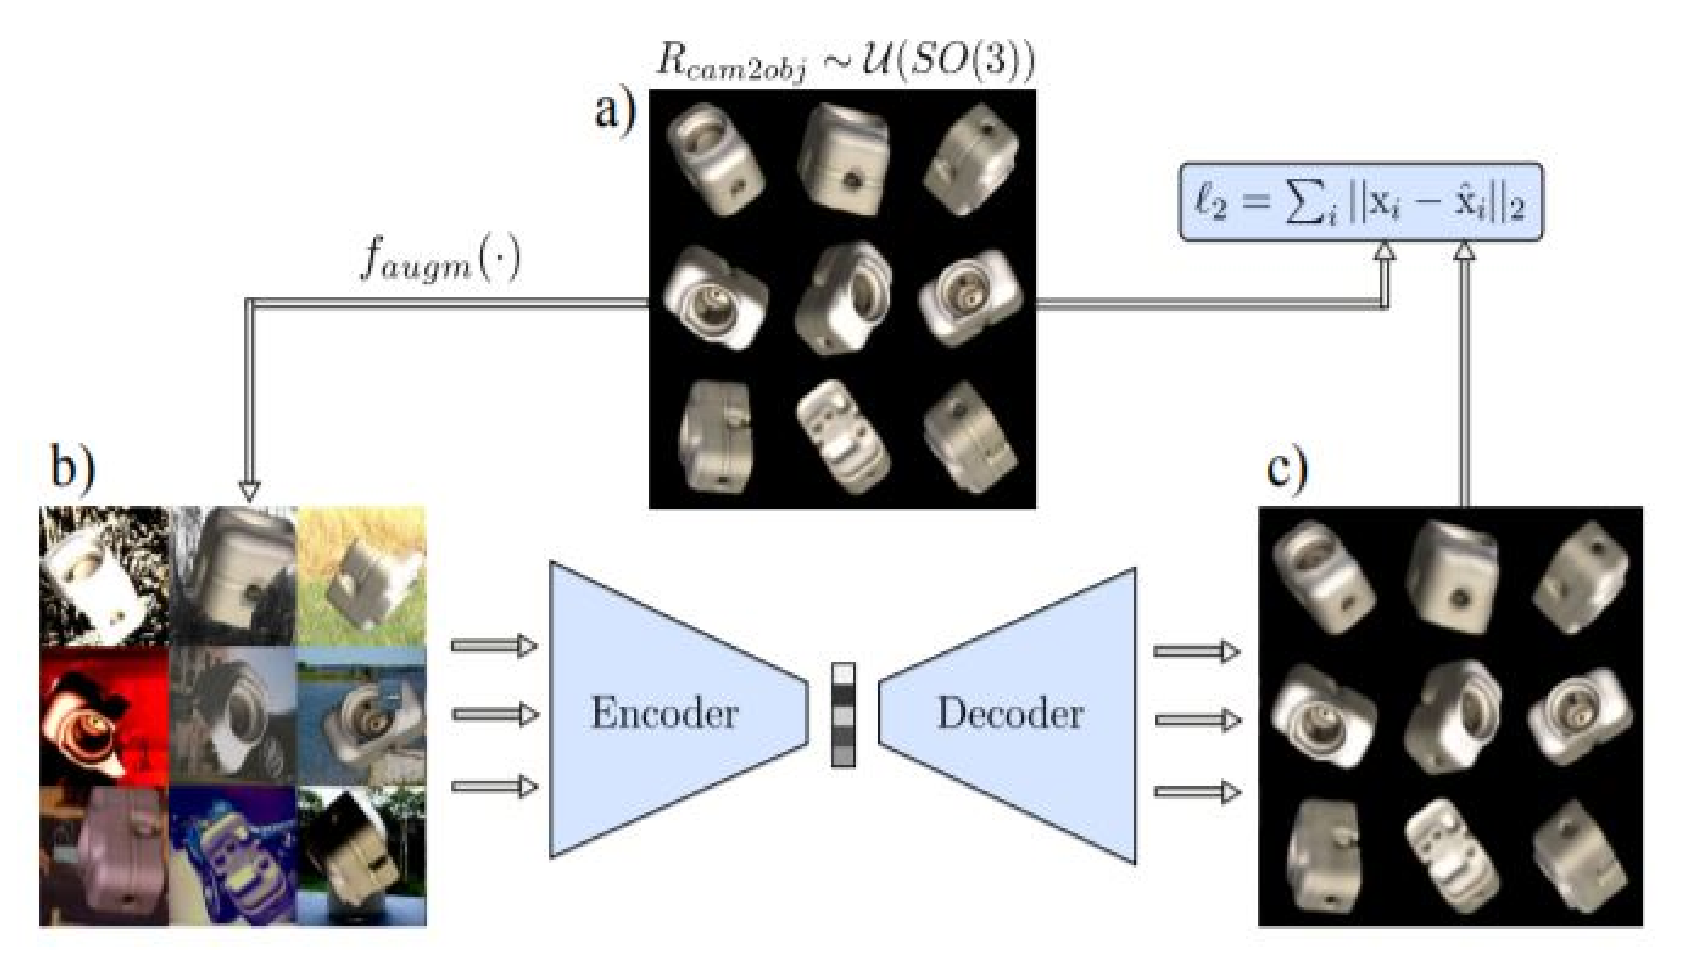
\includegraphics[width=100mm]{11-1.eps}
      \vspace*{25mm}
      \caption{AAEの概要.}
      \label{style1}
      \end{figure}

\subsubsection{トレーニング}
 入力画像サイズは128×128でチャンネル数3としてエンコード・デコードを行う.92232通りの姿勢画像を学習しそれぞれの潜在変数を取得する.

\subsubsection{推定}
 SSDにより物体を検出し検出したバウンディングボックスを切り抜きエンコーダに入力する,出力された潜在変数とトレーニング時に取得した潜在変数をK近傍法で最も近い値のものを物体姿勢として推定する.トレーニングから推定の流れを図\ref{style2}に示す.
 


      \begin{figure}[htpp]
      \centering
      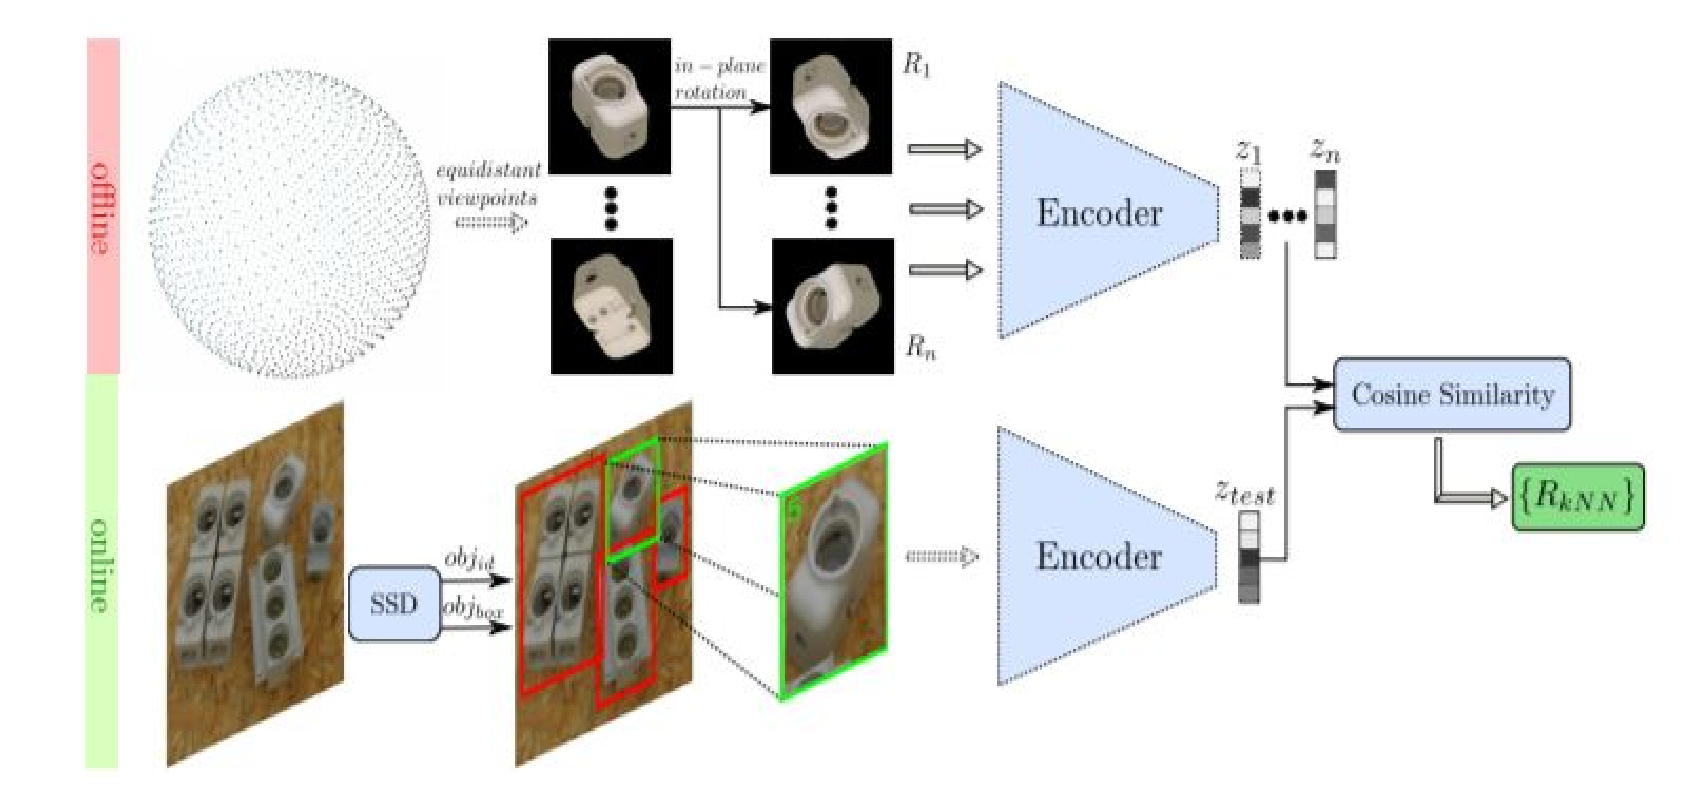
\includegraphics[width=100mm]{11-2.eps}
      \vspace*{25mm}
      \caption{トレーニング・推定.}
      \label{style2}
      \end{figure}


%----------------------------------------------------------------------------------------------------------------------------------------------------------

\subsection{pytorch版AAE}
 これまで論文元のGit-hubのコードでの実装を考えて進めてきたが,今後進めていくうえでAAEを自作での実装を行った方が良いと考えた.そこで現在pytorchでのAAEの実装を三輪が行っていたためデータをもらいそこからARマーカの姿勢推定を行えるものに作成していくこととなった.pytorch版での動作環境を表\ref{operating_environment}に示す\\


\begin{table}[H]
\caption{動作環境.}
\label{operating_environment}
\begin{center}
\begin{tabular}{c|c}
\hline
OS & Ubuntu 16.04 \\ \hline 
GPU & GeForce GTX 1060 \\ \hline
言語 & Python 3.5.2 \\ \hline
ライブラリ & pytorch 1.3.1\\ \hline
\end{tabular}
\end{center}
\end{table}

%----------------------------------------------------------------------------------------------------------------------------------------------------------

%---------------------------------------------------------------------------------------------------------------------------------------------------------

\subsection{モデル画像の用意}
 AAEを実装するにあたって自作モデルを用意し撮影する必要がある.トレーニングに用いるモデルは,円柱にARマーカを添わすように張り付けたmodel図\ref{style3}と円柱に平面状のARマーカをつけたmodel\ref{style4}の2つを用意する.トレーニング画像の作成はmodel作成をblenderを用いてmodelの撮影をgazeboを用いて用意する.

      \begin{figure}[htpp]
      \centering
      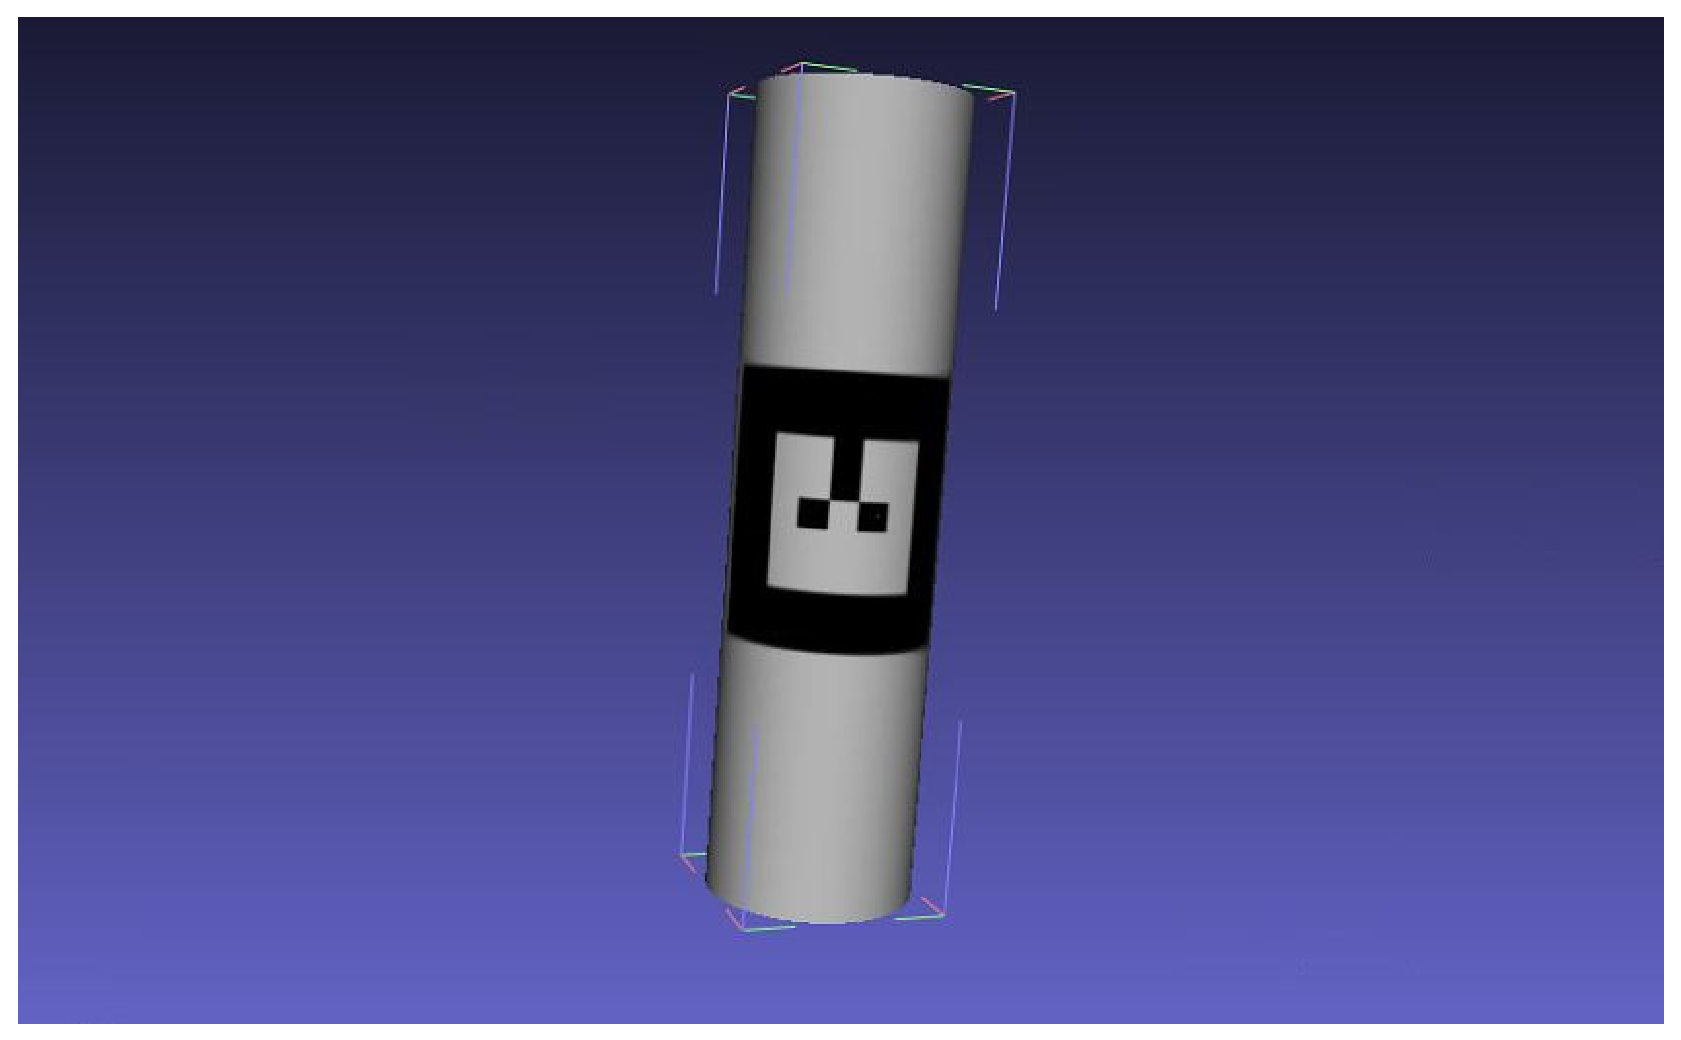
\includegraphics[width=100mm]{11-3.eps}
      \vspace*{25mm}
      \caption{model1.}
      \label{style3}
      \end{figure}

      \begin{figure}[htpp]
      \centering
      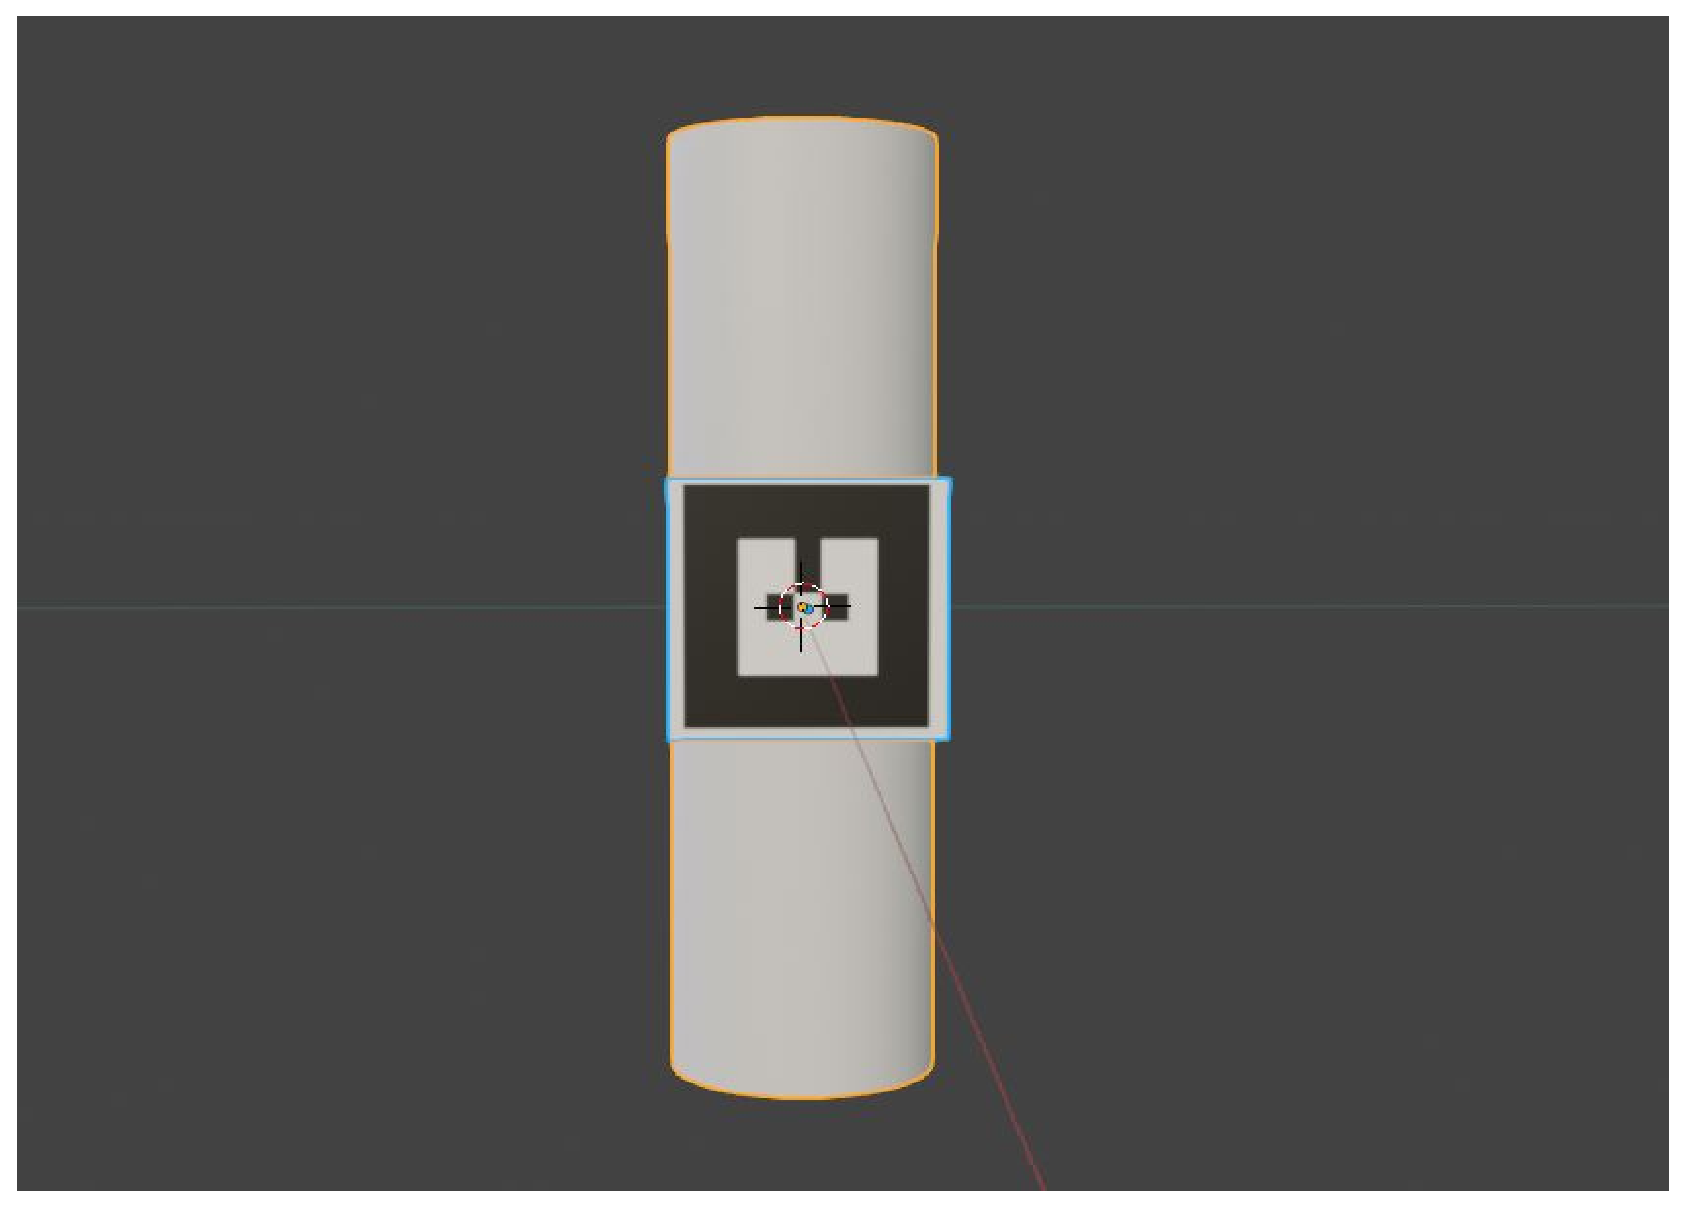
\includegraphics[width=100mm]{11-4.eps}
      \vspace*{25mm}
      \caption{model2.}
      \label{style4}
      \end{figure}






%---------------------------------------------------------------------------------------------------------------------------------------------------------
\section{おわりに}
 これまで,AAEの元論文のコードを実装しようとしていたが問題が多く自分では解決できないという時間が続いてしまい研究という点ではあまり進んでいなかったのでペース的にも遅れていると思われる.そのため現在やることが明確になったので一つ一つ明確になったやるべきことを早く終わらせ,考える作業に時間をさけるようにプログラムやモデルの作成などはより一層スピードを上げて終わらせていきたいと思う.

%---------------------------------------------------------------------------------------------------------------------------------------------------------

\footnotesize
\begin{thebibliography}{99}

\bibitem{fasterrcnn}
S.Ren {\em et al. }: ``Faster R-CNN: Towards Real-Time Object Detectionwith Region Proposal Networks'', Proc. of NIPS,2015.


\bibitem{Implicit 3D Orientation Learning for 6D Object Detection from RGB Images}
Martin Sundermeyer Zoltan-Csaba Marton Maximilian Durner Rudolph Triebel {\em et al. }:''Implicit 3D Orientation Learning for 6D Object Detection from RGB Images''  EVCC2018 




\end{thebibliography}

\normalsize

\end{document}